\colorlet{punct}{red!60!black}
\definecolor{delim}{RGB}{20,105,176}
\colorlet{numb}{magenta!60!black}

\lstdefinelanguage{json}{
	basicstyle=\normalfont\ttfamily,
	stepnumber=1,
	numbersep=8pt,
	showstringspaces=false,
	breaklines=true,
	frame=lines,
	backgroundcolor=\color{white},
	literate=
	*{0}{{{\color{numb}0}}}{1}
	{1}{{{\color{numb}1}}}{1}
	{2}{{{\color{numb}2}}}{1}
	{3}{{{\color{numb}3}}}{1}
	{4}{{{\color{numb}4}}}{1}
	{5}{{{\color{numb}5}}}{1}
	{6}{{{\color{numb}6}}}{1}
	{7}{{{\color{numb}7}}}{1}
	{8}{{{\color{numb}8}}}{1}
	{9}{{{\color{numb}9}}}{1}
	{:}{{{\color{punct}{:}}}}{1}
	{,}{{{\color{punct}{,}}}}{1}
	{\{}{{{\color{delim}{\{}}}}{1}
	{\}}{{{\color{delim}{\}}}}}{1}
	{[}{{{\color{delim}{[}}}}{1}
	{]}{{{\color{delim}{]}}}}{1},
}

\begin{quote}
In the Appendix we can put code snippets, snapshots,
installation instructions, etc.
\end{quote}
\subsection{Akka: configurazione Actor Systems}
\label{sec:akkaconf}
Ogni Actor System viene creato con le seguenti configurazioni:
\begin{itemize}
	\item ogni attore deve permettere la serializzazione di oggetti;
	\item la comunicazione è orientata alla connessione, infatti viene utilizzato il protocollo TCP;
	\item l'host sulla quale verrà eseguita l'applicazione è 127.0.0.1\footnote{Essendo la nostra implementazione una simulazione di un sistema distribuito l'host è unico e coincide con \texttt{localhost}; in contesti reali gli host corrispondono ad ogni macchina connessa alla rete. } e la prima porta che verrà occupata è la 2551;
	\item attraverso l'opzione \texttt{multi-mbeans-in-same-jvm = on} informiamo il sistema che su un unico host potranno essere eseguite più JVM; una per ogni Actor System.
\end{itemize}
\begin{lstlisting}[language=json]
akka {
  actor {
    provider = "cluster"
    warn-about-java-serializer-usage = false
    serialize-messages = on
    allow-java-serialization = on
  }
  remote {
   transport = "akka.remote.netty.NettyRemoteTransport"
   log-remote-lifecycle-events = off
   netty.tcp {
      hostname = "127.0.0.1"
      port = 2551
      }
  }

  cluster {
    jmx {
      multi-mbeans-in-same-jvm = on
      }
    seed-nodes = [
      "akka.tcp://ClusterSystem@127.0.0.1:2551"]
    }
}
\end{lstlisting}

\subsection{Akka: recovery mode}
\label{sec:akkarecovery}
Di seguito il codice sorgente in Java per la gestione delle eccezioni \emph{Channel Exception}:
\begin{lstlisting}[language=java]
public class DSCluster {
  private Integer numRobots;
  private int portSeed = 2551;
  private static final int maxRecovery = 5;
  
  private void actorSystemInitialization() {
    try {
      // Create Robot's ActorSystem.
      for (int i = 0; i < numRobots; ++i)
        actorSystemArray.add(ActorSystem.create("ClusterSystem",
          ConfigFactory.parseString("akka.remote.netty.tcp.port="
          + (portSeed + i)).withFallback(config)));
      view.showInformationMessage("AKKA: Every Robot is connected");
      robotMainActorInitialization();
    } catch (ChannelException e) {
      exceptionFound();
      portSeed += numRobots;
      for (int i = 0; i < actorSystemArray.size(); ++i) 
        actorSystemArray.remove(i);
      actorSystemInitialization();
    }
  }
  
  private void exceptionFound(){
    if (this.maxRecovery<actualRecovery) {
      JOptionPane.showMessageDialog(view.getMainFrame(),
      "The error recovery procedure failed.\n" +
      "The system is corrupt. Self-destruction activated!",
      "Adios !",
      JOptionPane.ERROR_MESSAGE);
      application.exit();
    }
    if(actualRecovery==0)
      view.showErrorMessage("AKKA: Error in cluster initialization."+
      "Starting recovery mode.");
    ++actualRecovery;
  }
}
\end{lstlisting}
La funzione \emph{actorSystemInitialization} prova a connettere uno alla volta gli Actor System nelle porte designate. Il primo sarà connesso alla porta \emph{portSeed}, mentre l'ultimo sarà connesso alla porta \emph{portSeed+numRobots}.
Nel caso venissero lanciate delle eccezioni del tipo \emph{Channel Exception}, l'utente verrebbe informato, \emph{portSeed} verrebbe incrementato di un numero d'unità pari a \emph{numRobots},  e gli Actor System eventualmente creati verrebbero eliminati. Dopo di che si ripartirebbe con la procedura di inizializzazione.
\subsection{Akka: creazione di un nuovo attore}
\label{sec:akkanew}
Di seguito il codice sorgente in Java per la definizione di un nuovo attore.
\begin{lstlisting}[language=java]
import akka.actor.*;

public class newActor extends AbstractActor {

  //Constructor whit two parameters
  public newActor(String str, CustomClass cs){
    //Initialize attributes
  };

  @Override
  public void preRestart(Throwable reason) {
   //Do something before the initialization
  }
  
   @Override
  public void postRestart(Throwable reason) {
    //Do something after the preRestart
  }
  
  @Override
  public void postStop(Throwable reason) {
    //Release the resource
  }
  
  @Override
  public Receive createReceive() {
    return receiveBuilder()
      .match(SomeClass.class, x -> {
        //Do something with x;
      })
      .match(AnotherClass.class, x->{
        //Do something with x
      })
    .build();
  
  static public Props props(String str, CustomClass cs) {
    return Props.create(newActor.class, str, cs);
  }
}
\end{lstlisting}

\subsection{Swing: implementazione della view}
\label{sec:view}
Nella seguente sezione verranno descritti alcuni screenshoot dell'applicativo.
\begin{figure}
\hspace{-2.5cm}
\includegraphics[scale=0.30]{immagini/inizioQuery.png}
\caption{La view principale descritta nella Sezione \ref{sec:viewImpl}.
In basso il log di sistema. A sinistra la visualizzazione dello stato di ogni query.
Nel centro la topologia del grafo principale.}
\end{figure}
\begin{figure}
	\centering
	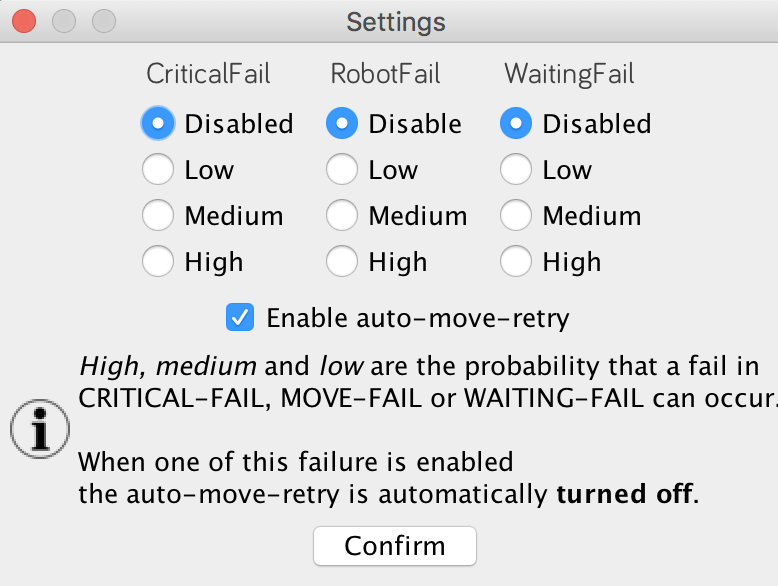
\includegraphics[scale=0.25]{immagini/settings.png}
	\caption{Impostazioni di sistema utilizzate per simulare i fallimenti.}
\end{figure}
\begin{figure}
	\hspace{-2.5cm}
	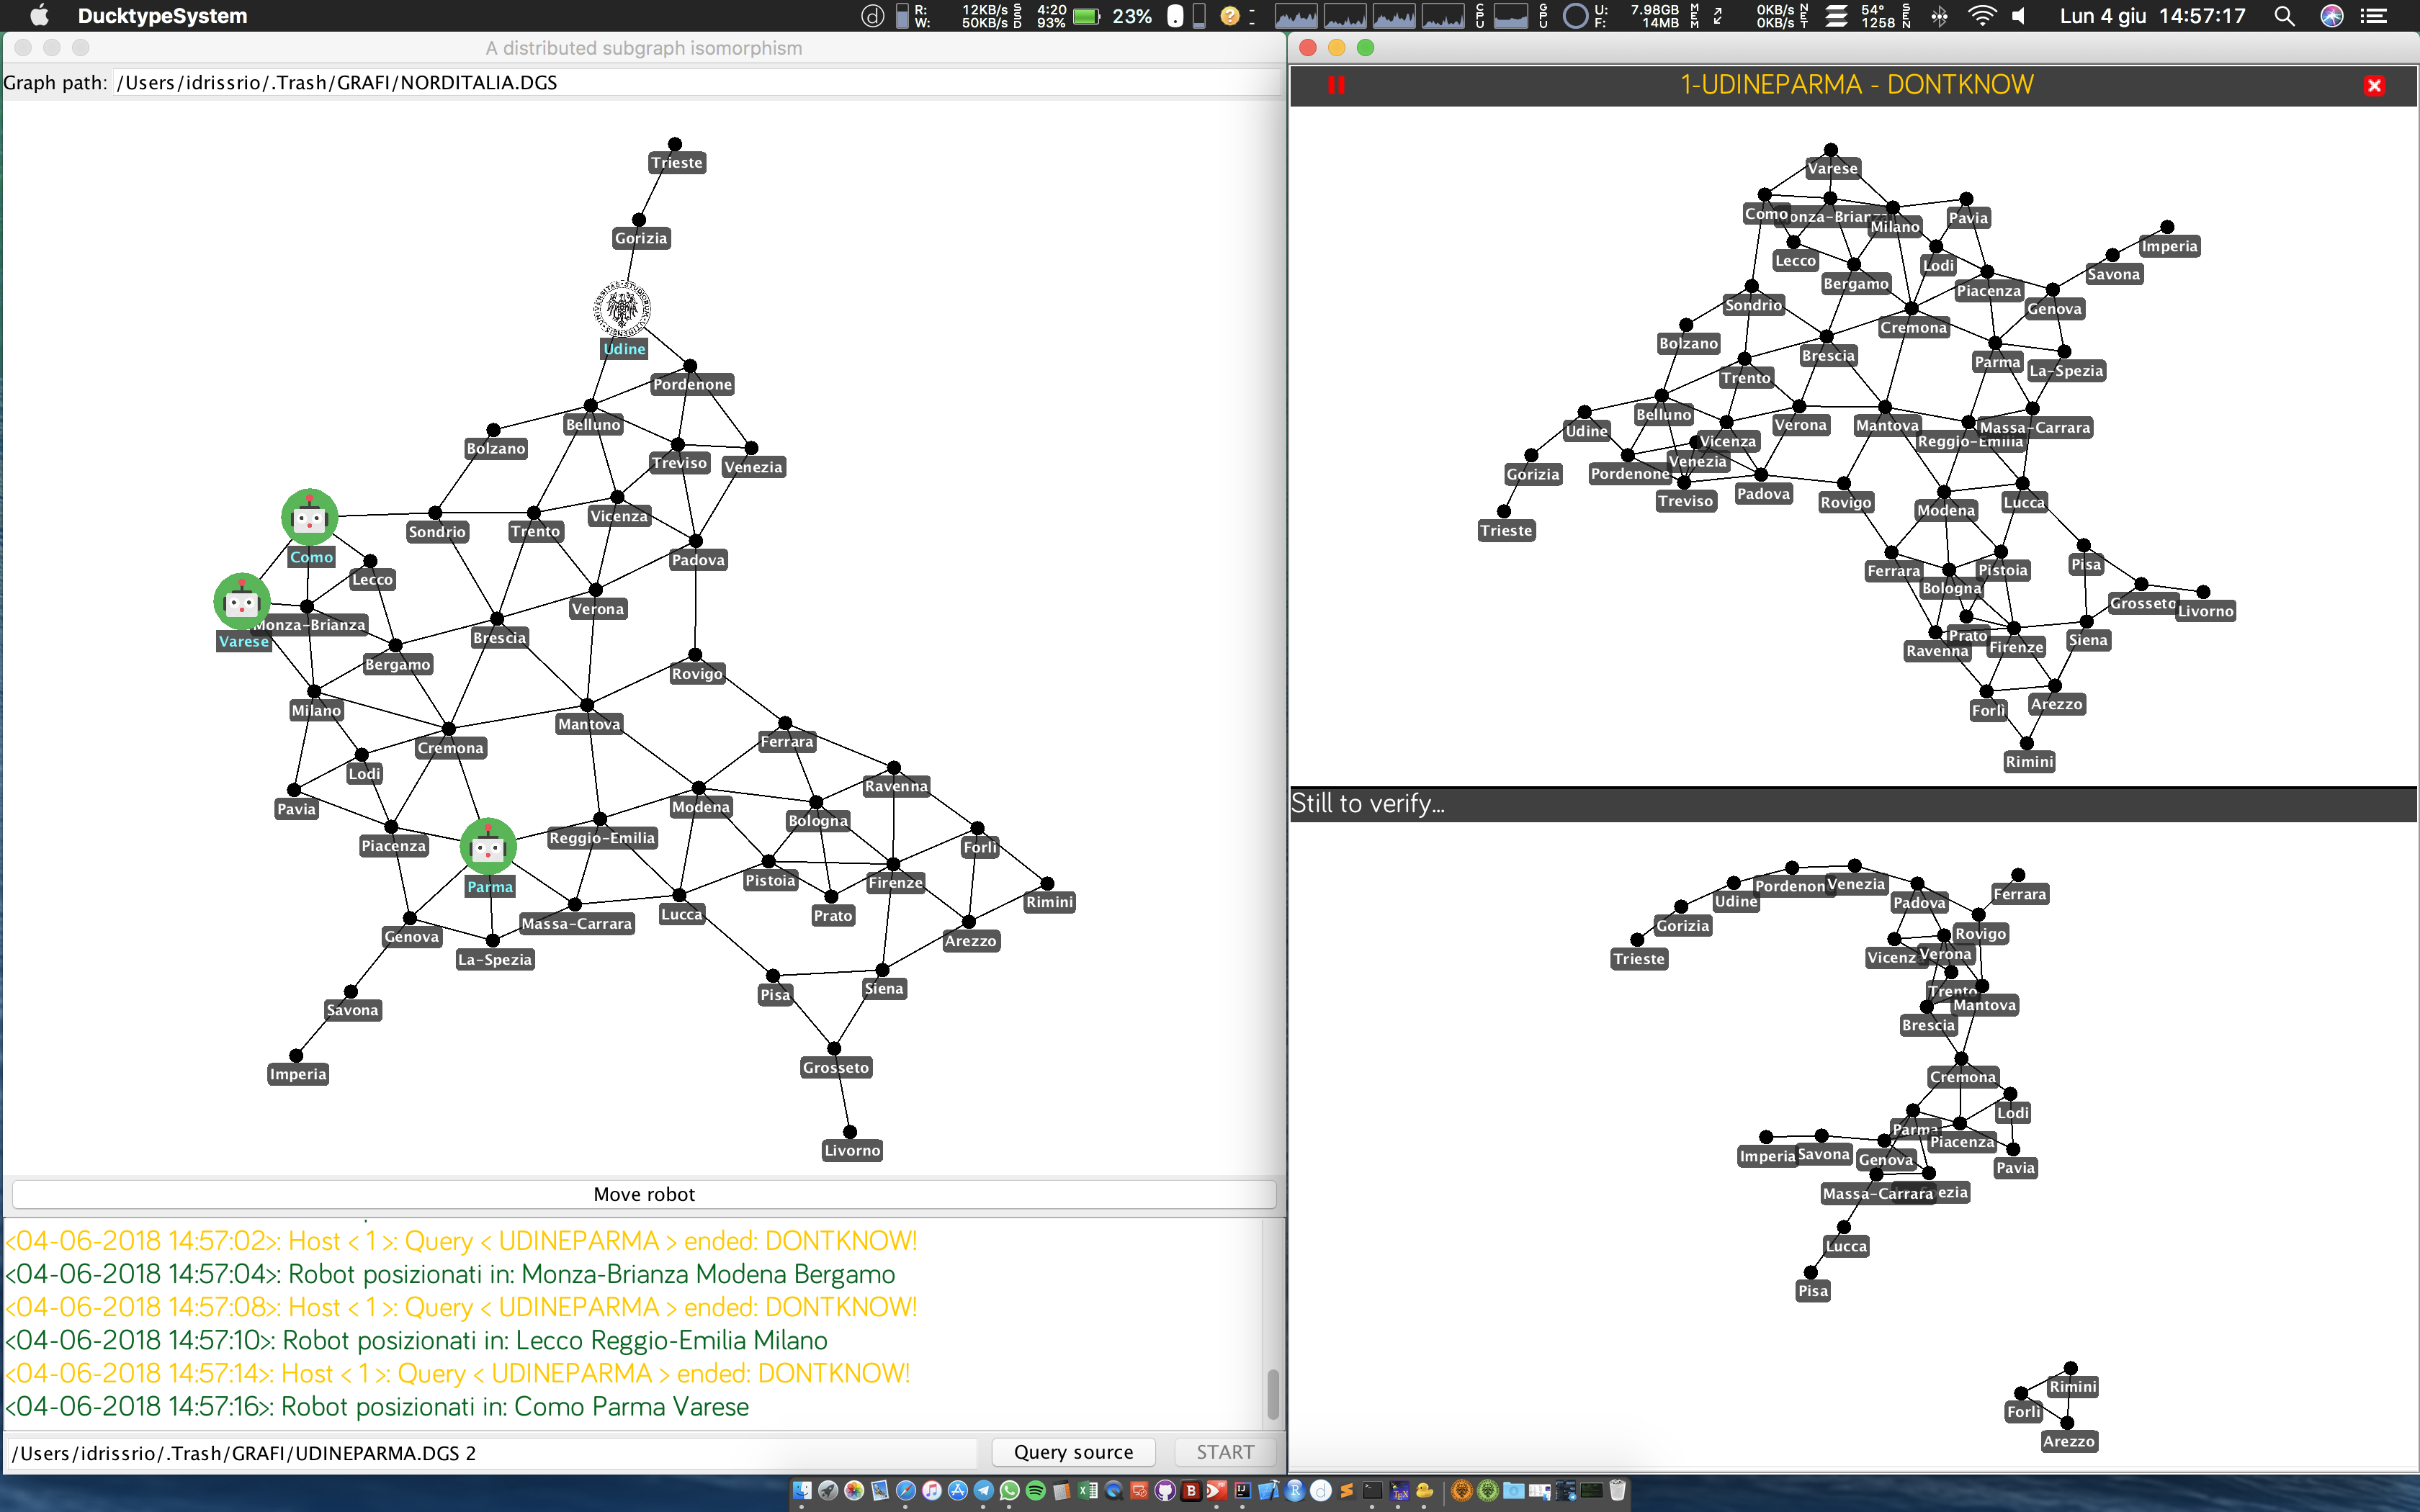
\includegraphics[scale=0.3]{immagini/betterVisualization.png}
	\caption{Modalità \emph{better visualization}: essendo alcuni grafi molto grandi, è stata introdotta la possibilità di scorporare il \emph{JPanel} di destra in una finestra a sè stante, permettendo una migliore visualizzazione delle query.}
\end{figure}


